\newcommand{\figpath}{Figures}
\newcommand{\totalRows}{6547}
\newcommand{\totalJavaRows}{4239}
\newcommand{\totalJavaScriptRows}{2308}
\newcommand{\totalDiscardedRows}{2985}
\newcommand{\javaDiscardedRows}{2126}
\newcommand{\jsDiscardedRows}{859}
\newcommand{\totalDeletedFiles}{432}
\newcommand{\remainingJavaFileCount}{2113}
\newcommand{\remainingJsFileCount}{1449}
\newenvironment{code}{\captionsetup{type=listing}}{}
\SetupFloatingEnvironment{listing}{name=Source Code}

\chapter{Solution Design and Implementation}\label{sec:design-and-impl-parent}
\section{Solution Design}\label{sec:design}
%%%%%%%%%%%%%%%%%%%%%%%%%%%%%%%%%%%%%%%%%%%%%%%%%%%%%%%%%%%%%%%%%%%%%%%%%%%%%%%%%%%%%%%%%%%%%%%%%%%%%%%%%%%
\subsection{Data Gathered}\label{sec:data-available}
The data collected contained \totalRows{} initially collected in 67 columns. Each record corresponds to a source code file at a given point in time and subsection \ref{sec:data-available} depicts attributes definition through Tables \ref{tbl:available-data-non-repeating-types} to \ref{tbl:available-data-above-0-max-100}, specifying uncommon datatypes found, as well as lists where each attribute in the list has the same properties with regards to data category, data type, and minimum and maximum values present. 

\begin{table}[h!]
\caption{Data Available - non repeating data types}
\label{tbl:available-data-non-repeating-types}
\begin{tabular}{@{}ll@{}}
\toprule
Metric name & Description \\ \midrule
issue key & text \\ 
file path & text \\
source repo & text \\
author & discrete, enumeration of possible authors \\
prev author & discrete, enumeration of possible authors\\
timestamp & continuous, epoch time \\
prev timestamp & continuous, epoch time \\
is bug & boolean, True or False \\
files & ordinal, integer, $\geq{}1$ \\
sqale debt & ratio, integer, $\geq{}0$ \\
statements & ordinal, integer, $\geq{}1$ \\
violations & ratio, integer, $\geq{}0$ \\ \bottomrule
\end{tabular}
\end{table}

\begin{table}[h!]
\caption{Ordinal data, integer, min $\geq{}0 \leq{}100$}
\label{tbl:available-data-above-0-max-100}
\begin{tabular}{@{}l@{}}
\toprule
Metric Name \\ \midrule
branch coverage \\
overall branch coverage \\
overall coverage \\
overall line coverage \\
overall uncovered conditions \\
overall uncovered lines \\ \bottomrule
\end{tabular}
\end{table}


\begin{table}[h!]
\caption{Numeric data, integer, min $\geq{}0$, no definitive maximum}
\label{tbl:available-data-above-0-no-max}
\begin{tabular}{@{}ll@{}}
\toprule
Metric Name & Metric Name \\ \midrule
blocker violations & line coverage \\
bugs & lines \\
classes & lines to cover \\
code smells & major violations \\
comment lines & minor violations \\
comment lines density & ncloc \\
complexity & open issues \\
confirmed issues & public documented API density \\
coverage & public undocumented API \\
critical violations & reliability rating \\
duplicated blocks & reliability remediation effort \\
duplicated files & reopened issues \\
duplicated lines & security rating \\
duplicated lines density & security remediation effort \\
effort to reach maintainability rating A & skipped tests \\
false positive issues & SQALE index \\
file complexity & SQALE rating \\
function complexity & test errors \\
functions & test failures \\
generated lines & test success density \\
generated ncloc & uncovered conditions \\
info violations & uncovered lines \\
it coverage & vulnerabilities \\
it line coverage & wont fix issues \\
it uncovered lines &  \\ \bottomrule
\end{tabular}
\end{table}


\subsection{Data Gathering Components}
The dataset for the analysis had to be generated from live business data as such data has not been made available in the public domain. Section \ref{sec:data-available} can be used a reference as to what metrics, along with their type and brief description, have been gathered. In order to construc the dataset subsequently used in the analysis, 3 real live business tools were used:

\begin{enumerate}{\label{lst:tools_used}}
    \item Sonar server by SonarSource - provided code quality metrics
    \item JIRA by Atlassian  - provided information about file commits as well as the classification of commits into "a bug" or "not a bug" categories
    \item Bitbucket by Atlassian  - provided information about commit timestamp, the author as well as details about previous commit author and previous commit timestamp allowing for calculating file staleness 
\end{enumerate}
    
Additionally, a tool to gather metrics, referred to as Data Gatherer, has been developed in order to produce the end dataset and will be made available upon submission. The purpose of the Data Gatherer tool is to coordinate the execution of other tools from the above list as well as collate the acquired data into the end dataset then used in further analysis as per Figure \ref{fig:data_gathering}.

\begin{figure}[h!]
\centering
    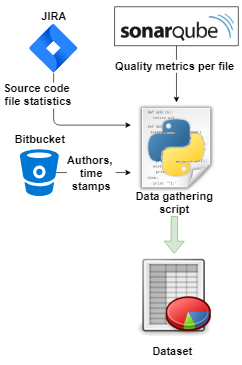
\includegraphics{\figpath/data_arch_small.png}
    \caption{Dataset Gathering operations}
    \label{fig:data_gathering}
\end{figure}

First tool to be used in the data gathering process is Atlassian's JIRA server. JIRA is a ticketing system used by software developers to keep track of issues, feature requests and most importantly in the current context, bugs. Each ticket has been assigned a category upon its creation depicting its purpose. In the context of the current use case the most relevant types encountered are:

\begin{itemize}
    \item Story - represents a feature task to be done. Upon completion it is a fully functional, testable vertical slice of functionality delivering value to end-users
    \item Task - represents an additional development task, such as, but not limited to, setting up test environments, automatization of effort, including testing effort, infrastructure maintenance etc. Does not provide direct value to end users
    \item Bug - represents issues found in released software, especially when expected and actual behaviour of a given piece of functionality doesn't match.
\end{itemize}
Given that Task type tickets are not directly linked to the development life cycle they have been excluded from further analysis and the focus has been placed on Story and Bug type tickets instead.

The second use of JIRA server was its proprietary integration with the source code repository - Bitbucket, as both tools are offered by the same company, Atlassian. For each of the JIRA tickets there existed a link between a given ticket and source code file changes, or commits, made and persisted in Bitbucket system. 
Each commit could consist of many files and each source code file could have been committed to multiple times under the umbrella of a single ticket. However, not all commit records under a ticket have been taken into the account - every so called merge commit have been excluded.

To illustrate what a merge commit is and why it must be excluded \ref{fig:git-branching-merging-and-rebasing} will be used, where blue nodes signify the master, or the golden copy of the code, and green and purple identify branches, where feature, bug fix or any other development work is carried out as part of a development lifecycle. At the end of its life a branch will be integrated into the Master branch, which will generate a merge commit - illustrated by Feature 1 branch. Additionally, it is a normal occurrence to have more than 1 branch created in a given codebase at any given time. If another branch has been created from the master before Feature 1 code was merged, as per \ref{fig:git-branching-merging-and-rebasing} Feature 2, and it is actively being developed on past the merge point such branch will have to be rebased. The rebase process will pull in the merge commit created by Feature 1, however, all source code files listed under merge commit will have already been analyzed under JIRA ticket representing Feature 1, therefore should it not be excluded from further analysis it would have duplicated the effort. Not excluding merge commits also represented significant risk with regards to story vs. bug categorization of source code files committed as Feature 2 might as well have been a bug. In such scenario file committed under Feature 1 ticked would be categorized as non-bug, as per ticket category, as well as bug as per category assigned by the second ticket.

\todo{Need to change Feature 2 to Bug, to illustrate merge commit exclusion better}
\begin{figure}[!h]
    \centering
    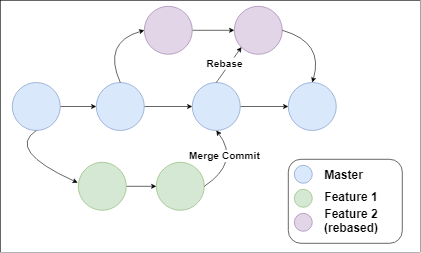
\includegraphics{\figpath/git_branching.png}
    \caption{GIT branching and rebasing strategy}
    \label{fig:git-branching-merging-and-rebasing}
\end{figure}

JIRA ticketing system provided the following columns:
\begin{itemize}
    \item issue key
    \item source repository
    \item file path
    \item category of the record, bug or not a bug
\end{itemize}

while the Bitbucket server provided additional information about:
\begin{itemize}\label{lst:design:info-from-bitbucket}
    \item author
    \item previous author
    \item commit timestamp
    \item timestamp of the previous commit
\end{itemize}

The final tool utilized was SonarQube by SonarSource, an open-source platform. Its capabilities include continuous inspection of code quality to perform automatic reviews with static analysis of code to detect code smells, reports on duplicated code, coding standards, unit tests, code coverage, code complexity, comments,  security vulnerabilities, and much more. In the context of this use case it was utilized to associate code metrics listed in Tables \ref{tbl:available-data-above-0-max-100} and \ref{tbl:available-data-above-0-no-max} as well as \texttt{files}, \texttt{sqale debt}, \texttt{statements} and \texttt{violations} provided in Table \ref{tbl:available-data-non-repeating-types}.

The \texttt{issue key}, \texttt{source repository} and \texttt{file path} were only used to verify that a given data point can be traced to a relevant JIRA ticket in order to verify it belongs to a assigned category, \texttt{author} and \texttt{previous author} were used to populate seniority and project tenure features, \texttt{timestamp} and \texttt{previous timestamp} were used to calculate staleness of the file between changes.



\subsection{Data Modelling}

Once a dataset has been generated as per section \ref{sec:design} it underwent the following operations:
\begin{enumerate}\label{lst:dataset-ops}
    \item missing data analysis and data cleaning \label{lst:dataset-ops.item:data-cleaning}
    \item balance of bug to non-bug records in the dataset \label{lst:dataset-ops.item:bug-to-non-bug-balance}
    \item outlier analysis \label{lst:dataset-ops.item:outliers}
    \item data correlation analysis \label{lst:dataset-ops.item:data-correlation}
    \item feature transformation \label{lst:dataset-ops.item:feature-transformation}
    \item feature scaling \label{lst:dataset-ops.item:data-scaling}
    \item relevant feature selection \label{lst:dataset-ops.item:feature-selection}
    \item distribution of selected features \label{lst:dataset-ops.item:attribute-distribution}
    \item evaluation of regularized Logistic Regression model \label{lst:dataset-ops.item:ml-logistic-regression}
    \item evaluation of Decision Tree Classification model \label{lst:dataset-ops.item:ml-decision-tree}
    \item evaluation of additional models as necessary \label{lst:dataset-ops.item:ml-models-additional}
\end{enumerate}

Item \ref{lst:dataset-ops.item:data-cleaning} focuses on cleaning and imputing values for missing metrics. Item \ref{lst:dataset-ops.item:bug-to-non-bug-balance} will focus on listing the ratios between bug and non bug records in the dataset.
Item \ref{lst:dataset-ops.item:outliers} identifies if there are any projects or individual files that are diverging significantly from the rest of the dataset. 
Item \ref{lst:dataset-ops.item:data-correlation} focuses on identifying any feature correlation patterns in order to proceed with feature selection - item  \ref{lst:dataset-ops.item:feature-selection} after which it will be necessary to check for the balance and distribution of the selected features or attributes - which will be the focus of item \ref{lst:dataset-ops.item:attribute-distribution}. Feature distribution is included as part of the analysis as Logistic Regression model is susceptible to non-normally distributed datasets.
Item \ref{lst:dataset-ops.item:data-scaling} concentrates on evaluating multiple scaling methods with regards to their effectiveness of bringing the dataset values to the same scale of magnitude. The scaling method taken into the account are:
\begin{enumerate}
    \item Transformation using natural logarithm - $log(e)$ 
    \item Min-Max scaling
    \item Max-Abs scaling
    \item Standard scaling
    \item Power Transformation using Yeo-Johnson variant
    \item Quantile Transformation using uniform distribution variant
    \item Quantile Transformation using normal distribution variant
\end{enumerate}

\todo{Probably need to talk a bit about what each scaler does and how it works. However, maybe it's better served in the implementation section}
Finally, an evaluation of the effectiveness of selected machine learning models with regards to predicting bug vs non-bug classes in the dataset will be carried out and constitutes the focus of items \ref{lst:dataset-ops.item:ml-logistic-regression}, \ref{lst:dataset-ops.item:ml-decision-tree} and \ref{lst:dataset-ops.item:ml-models-additional} respectively.

\section{Implementation}\label{sec:implementation}
The implementation has been carried out in two steps. In the first step, a tool has been developed in Python language for the purpose of gathering the data required for the analysis - the process is outlined in Section \ref{sec:impl-data-gatherer}. Secondly, the data has been analyzed, in accordance with steps defined in Section \ref{sec:design}, List \ref{lst:dataset-ops}, using Jupyter Notebook tooling, which is the topic of Section \ref{sec:impl-data-analysis}.

\subsection{Data Gatherer}\label{sec:impl-data-gatherer}
The data gatherer tool has been split into a number of files for readability and maintenance. Additionally significant portion of the code written has been tested with automated tests. Project structure is initially split between source code and test code folders, named \texttt{src} and \texttt{test} respectively. In each a number of resource files have been defined to support the program execution, mock server responses and data or provide additional information. Source folder structure has been illustrated on Figure \ref{fig:impl-data-gatherer-source-files}.
\begin{enumerate}
    \item \texttt{gatherer\_main.py} - included in full in code excerpt \ref{code:gatherer_main.py}. Coordinates all data gathering operations. 
    \item\label{lst:impl.item:jira} \texttt{jira\_connector.py} - Handles all communication and authentication with a given JIRA server. From a list of JIRA keys contained in \texttt{bug\_issue\_key\_list.dat} and \texttt{story\_issue\_key\_list.dat} interrogates the server over REST API to obtain an ID attribute for each ticket. Then, again using JIRA's REST API, obtains a list of commits for a given JIRA ID for all code repositories. 
    
    At this step a number of infrastructure repositories that are maintenance only, or ones that are written in languages not supported by Sonar server, thus making it impossible to obtain code quality metrics, have been removed.
    
    In the next step all merge commits are being removed from the analysis as it would otherwise create duplicate data points. For detailed explanation refer to Section \ref{sec:design}. Additionally a number of files are removed from the analysis - for details on what file extensions were ignored as well as a brief reasoning for same, refer to Table \ref{tbl:file-extensions-excluded-from-analysis}.
    
    In the final step a list of initial metrics identifying a given commit is compiled. Alongside it, a map containing \texttt{issue\_key}, \texttt{source\_repository}, \texttt{commitId}, \texttt{path} and \texttt{repo\_code}, which is a unique 3-4 character abbreviation identifying a repository, is composed. Complete map containing both commit details as well as information necessary in the subsequent step is returned back to the coordinator file. 
    
    For code listing for this step refer to code exceprt \ref{code:jira-connector.py}
    
    \item\label{lst:impl.item:bitbucket} \texttt{bitbucket.py} - handles all communication and authentication with a given Bitbucket server. Given data provided by JIRA server from above item interrogates a specified Bitbucket server over REST API in order to obtain details of previous commit such as author and timestamp. As previously described in Section \ref{sec:design}, List \ref{lst:design:info-from-bitbucket} those details will be used in subsequent analysis steps to provide indication of developers' level of experience based on seniority as well as familiarity with a given product based on the amount of time spend on the project.
    
    Once all those details have been obtained an compiled they are returned to the coordinator file.
    Complete code listing is available from code excerpt\ref{code:bitbucket.py}.
    
    \item\label{lst:impl.item:sonar-metrics-gatherer} \texttt{sonar\_metrics\_gatherer.py} - is responsible for all communication via REST API with Sonar server instance. Using data gathered by JIRA and Bitbucket steps above it contacts Sonar server for each and every file, for each and every commit under each JIRA ticket and retrieves a specified list of code quality metrics. The list is defined in \texttt{sonar\_metrics\_enum.py} and it is comprehensive. 
    
    In order to retrieve code quality metrics first the expected parameters need to generated from data retrieved from both JIRA and Bitbucket - the expected data is called project component  and it is an unique identifier on Sonar Server for each file ever analyzed. The project component is in different format for some projects therefore it was necessary to model a number of generation use cases, as outlined in the \texttt{sonar\_component\_name\_generator} method in \ref{code:sonar-gatherer.py} code listing.
    
    One thing to note is that for different source code languages different metrics, especially with regards to the code coverage metrics can be provided by Sonar. For example for JavaScript based languages such as Angular JS there is a separate position for integration, or IT, coverage, whereas for Java and other JVM based languages that metric is rarely provided. In JVM based languages it has been folded into the \texttt{overall code coverage} metric instead.
    
    
    Once metrics have been gathered, they are combined with data gathered in previous steps and all information is output into a \texttt{results.csv} file representing complete dataset to be analyzed. For code listing for this step refer to code exceprt \ref{code:sonar-gatherer.py}
\end{enumerate}

\begin{table}[h!]
\centering
\caption{Files excluded from the analysis by extension or suffix}
\label{tbl:file-extensions-excluded-from-analysis}
\begin{tabular}{@{}ll@{}}
\toprule
Extension or Suffix & Reason for exclusion \\ \midrule
 &  \\
 &  \\
 &  \\
 &  \\ \bottomrule
\end{tabular}
\end{table}

\todo{need to remove the backup folder and then retake picture}
\begin{figure}[!h]
    \centering
    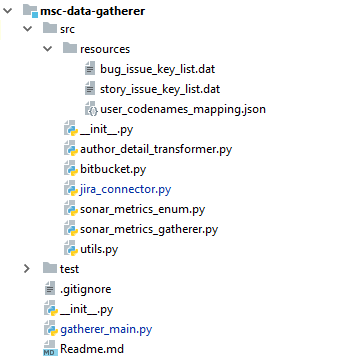
\includegraphics{Figures/impl_src_folder_files.png}
    \caption{Source Files}
    \label{fig:impl-data-gatherer-source-files}
\end{figure}


\begin{landscape}

\begin{code}
\captionof{listing}{Main data gathering component - the coordinator}
\label{code:gatherer_main.py}
\begin{minted}[breaklines]{python}
class Gatherer:

    def __init__(self):
        self.header_printed = False

    def main(self, username, password, jira_keys, is_bug_file):
        for jira_key in jira_keys:
            jira_obj = JiraConnector(username, password)
            # get metrics from JIRA
            files, commit_details = jira_obj.main(jira_key)

            sonar_obj = SonarMetricsGatherer(username, password)
            output = []
            bb = Bitbucket(username, password)
            # get information about previous commits
            prev_commit_details = bb.get_prev_commit_details_per_filepath(commit_details)
            # encode author's fullname for identity protection
            prev_commit_details = AuthorDetailsTransformer().transform_names_into_codenames(prev_commit_details)

            for file in files.keys():
                repo_file_is_in = files[file]
                component_key = sonar_obj.get_project_key_by_project_name(repo_file_is_in)

                # check if component key was generated correctly
                if len(component_key) <= 0:
                    self.log_jira_error(jira_key)
                    continue

                # get component_name
                component_name = sonar_obj.sonar_component_name_generator(component_key, file)
               
                # check if component name was generated correctly
                if len(component_name) <= 0:
                    self.log_jira_error(jira_key)
                    continue

                sorted_metrics_dict = sonar_obj.main(component_name, repo_file_is_in)
               
                # check if metrics were generated correctly
                if len(sorted_metrics_dict) > 0:
                    sorted_metrics_dict['source_repo'] = repo_file_is_in
                    sorted_metrics_dict['is_bug'] = is_bug_file
                    sorted_metrics_dict['issue_key'] = jira_key
                    combined = sorted_metrics_dict.copy()
                    combined.update(prev_commit_details[file])
                    output.append(combined)

                    sonar_obj.save_to_csv(header_printed=self.header_printed, list_of_metric_dicts=output,
                                          out_path='results.csv')
                    self.header_printed = True  # ensure that header is only appended once to target CSV
                else:
                    self.log_jira_error(jira_key)

    def log_jira_error(self, jira_key):
        print('Error with processing JIRA: {0}'.format(jira_key))

    def load_jira_key_files(self, file_location):
        values = []
        with open(file_location) as f:
            for line in f:
                line = line.replace('\n', '')
                values.append(line)
        return values


if __name__ == '__main__':
    start_time = time.time()
    urllib3.disable_warnings()
    username = None
    password = None
    if len(sys.argv) > 2:
        username = sys.argv[1]
        password = sys.argv[2]
    try:
        obj = Gatherer()
        # get data from bug tickets
        jira_keys = obj.load_jira_key_files('src/resources/bug_issue_key_list.dat')
        obj.main(username, password, jira_keys, True)

        # get data from regular tickets
        jira_keys = obj.load_jira_key_files('src/resources/story_issue_key_list.dat')
        obj.main(username, password, jira_keys, False)
        print('Operation duration: {0}'.format(time.time() - start_time))
    except Exception as e:
        print('Operation completed with an error. Duration: {0}'.format(time.time() - start_time))

\end{minted}
\end{code}



\begin{code}
\captionof{listing}{JIRA Connector - extracts relevant metrics from a given JIRA ticket}
\label{code:jira-connector.py}
\begin{minted}[breaklines]{python}
class JiraConnector:
    server_url_base = 'https://cksvnprd01.corp.emc.com/jira'
    url = 'https://cksvnprd01.corp.emc.com/jira/rest/webResources/1.0/resources'

    username = ''
    password = ''

    def __init__(self, username, password):
        self.username = username
        self.password = password

    def main(self, issue_key='ZZZ-1234'):
        issue_id = self.get_jira_id_from_jira_key(issue_key)

        resp = self.get_commit_details_for_a_jira_id(issue_id)
        return self.get_filenames_from_commits(resp)

    def is_valid_project(self, project_name):
        exclusions_pattern = '' # omitted for brevity
        exclusions_re = re.compile(exclusions_pattern)

        if exclusions_re.match(project_name):
            return False
        else:
            return True

    def get_jira_details_url(self, key):
        base_url = self.server_url_base + '/rest/api/2/issue/{0}'
        return base_url.format(key)

    def get_jira_id_from_jira_details(self, jira_details):
        id_key = 'id'
        return jira_details.get(id_key)

    def get_jira_id_from_jira_key(self, jira_key):
        url = self.get_jira_details_url(jira_key)

        jira_details_resp = requests.get(url, auth=HTTPBasicAuth(self.username, self.password), verify=False)
        if (jira_details_resp.status_code == 404):
            backup_url = 'https://cksvnprd01.corp.emc.com:4443/joanna/rest/api/2/issue/{0}'.format(jira_key)
            jira_details_resp = requests.get(backup_url, auth=HTTPBasicAuth(self.username, self.password), verify=False)
            print(backup_url)
            print(jira_details_resp.text)
        return self.get_jira_id_from_jira_details(jira_details_resp.json())


    def get_commit_details_for_a_jira_id(self, jira_id):
        resp = requests.get(self.get_commit_details_url(jira_id), auth=HTTPBasicAuth(self.username, self.password),
                            verify=False)
        return resp.json()

    def get_commit_details_url(self, id):
        url_base = self.server_url_base + '/rest/dev-status/1.0/issue/detail?issueId={0}&applicationType=stash&dataType=repository&_=1549641890823'
        return url_base.format(id)

    def get_repositories_from_json_response(self, json_details):
        repositories_section = json_details['detail'][0]['repositories']
        return repositories_section

    def get_repo_slug_from_repo_url(self, repo_url):
        slug_expr = re.compile('http.?://gssd-stash.isus.emc.com/projects/(\w+)\/.*')
        return slug_expr.match(repo_url).group(1)

    def get_commits_from_json_response(self, input_json):
        repositories_section = self.get_repositories_from_json_response(input_json)

        commits_in_repo = {}
        for repo in repositories_section:
            repo_name = repo['name']
            if self.is_valid_project(repo_name):
                repo_slug = self.get_repo_slug_from_repo_url(repo['url'])
                for commit in repo['commits']:
                    if commit['merge'] is False:

                        commit['repo_slug'] = repo_slug
                        if repo_name not in commits_in_repo.keys():
                            current_commits = [commit]
                            commits_in_repo[repo_name] = []
                            commits_in_repo[repo_name] = current_commits
                        else:
                            current_commits = commits_in_repo[repo_name]
                            current_commits.append(commit)
                            commits_in_repo[repo_name] = current_commits
        return commits_in_repo

    def get_filenames_from_commits(self, json):
        repo_to_commits_dict = self.get_commits_from_json_response(json)
        filenames = {}
        commit_details = {}
        java_exclusions = '' # omitted for clarity
        kotlin_exclusions = '' # omitted for clarity
        javascript_exclusions = '' # omitted for clarity
        other_exclusions = '' # omitted for clarity
        java_re = re.compile(java_exclusions)
        kotlin_re = re.compile(kotlin_exclusions)
        javascript_re = re.compile(javascript_exclusions)
        other_re = re.compile(other_exclusions)
        for repo in repo_to_commits_dict.keys():
            for commit in repo_to_commits_dict[repo]:
                for file in commit['files']:
                    if java_re.match(file['path']) or kotlin_re.match(file['path']) or javascript_re.match(
                            file['path']) or other_re.match(file['path']):
                        pass
                    else:
                        filenames[file['path']] = repo
                        commit_id = commit['id']
                        repo_slug = commit['repo_slug']
                        partial = {}
                        partial['commitId'] = commit_id
                        partial['target_repo'] = repo
                        partial['repo_code'] = repo_slug
                        commit_details[file['path']] = partial
        return filenames, commit_details

    def get_repo_name(self, json):
        return self.get_repositories_from_json_response(json)[0]['name']
\end{minted}
\end{code}

\begin{code}
 \captionof{listing}{Bitbucket connector - retrieves commit metrics for a given file}
 \label{code:bitbucket.py}
 \begin{minted}[breaklines]{python}
 class Bitbucket:
    bitbucket_url_sample = 'https://gssd-stash.isus.emc.com/rest/api/latest/projects/{0}/repos/{1}'\
    '/commits?followRenames=true&path={2}&until=refs%2Fheads%2Fdevelop&start=0&limit={3}'
    username = ''
    password = ''

    def __init__(self, username, password):
        self.username = username
        self.password = password

    def executor(self):
        resp = self.get_last_two_commits()
        if resp.status_code != 200:
            raise ApiError('Bitbucket server responded with {} code'.format(resp.status_code))

    def get_last_two_commits(self, project_key='CFG', project_name='oberon-asset-management',
                             project_file_path='', no_of_commits_to_pull=2):
        url = self.bitbucket_url_sample.format(project_key, project_name, project_file_path, no_of_commits_to_pull)
        resp = requests.get(url, auth=HTTPBasicAuth(self.username, self.password), verify=False)
        return resp

    def get_prev_commit_details_per_filepath(self, jira_details_json):
        url = 'https://gssd-stash.isus.emc.com/rest/api/1.0/projects/{0}/repos/{1}/commits/{2}'
        complete_results = {}
        for file in jira_details_json:
            result_items = {}
            item = jira_details_json[file]
            target_url = url.format(item['repo_code'], item['target_repo'], item['commitId'])
            resp = requests.get(target_url, auth=HTTPBasicAuth(self.username, self.password), verify=False)
            result = resp.json()
            author_name = result['author']['name']
            timestamp = result['authorTimestamp']
            parent_section = result['parents'][0]
            prev_author = parent_section['author']['name']
            prev_timestamp = parent_section['authorTimestamp']

            result_items['author'] = author_name
            result_items['timestamp'] = timestamp
            result_items['prev_author'] = prev_author
            result_items['prev_timestamp'] = prev_timestamp
            complete_results[file] = result_items
        return complete_results

 \end{minted}
 \end{code}
 
 \begin{code}
 \captionof{listing}{Sonar connector - retrieves code quality metrics for a given file}
 \label{code:sonar-gatherer.py}
 \begin{minted}[breaklines]{python}
 class SonarMetricsGatherer:
    username = None
    password = None

    def __init__(self, username, password):
        self.username = username
        self.password = password

    server_url = 'http://10.60.142.206:9000'
    component_api_url = '/api/measures/component?componentKey='
    metrics_to_pull = '&metricKeys=' # actual list of keys have been omitted for brevity

    def make_url(self, target_file, server_url=server_url, component_url=component_api_url, metrics=metrics_to_pull):
        return server_url + component_url + target_file + metrics

    def main(self, target_file, repo_name):
        url = self.make_url(target_file)
        resp = requests.get(url, auth=HTTPBasicAuth(self.username, self.password))
        metrics_map = {}
        if resp.status_code != 200:
            print('File that errored out: {0}'.format(target_file))
            # raise ApiError('Sonar server responded with {} code'.format(resp.status_code))
        else:

            resp_component = resp.json().get('component')
            formatted_file_path = self.format_target_file_path_for_display(target_file)

            metrics_map = self.filter_metrics(self.convert_metrics_to_map(resp_component))
            metrics_map['file_path'] = formatted_file_path

        return metrics_map

    def format_target_file_path_for_display(self, file_path):
        return file_path.replace('%3A', '/').replace('%2F', '/')

    def sonar_component_name_generator(self, component_key, file_name_from_jira):
        try:
            component, branch = component_key.rsplit(':', 1)
            module_name, path = file_name_from_jira.split('/', 1)
            test_url = ''
            if 'unified-ui' in component_key:
                test_url = component + ':' + branch + ':' + module_name + '/' + path
            else:
                test_url = component + ':' + module_name + ':' + branch + ':' + path
           
            return test_url.replace(':', '%3A').replace('/', '%2F')
        except ValueError:
            print('Couldn\'t generate name for component {0} filename {1}'.format(component_key, file_name_from_jira))
            return ''
        # %3A = :
        # %2F = /

    def search_for_project_by_name(self, project_name):
        search_url = 'http://10.60.142.206:9000/api/projects/index?search={0}%20develop'.format(project_name)
        resp = requests.get(search_url, auth=HTTPBasicAuth(self.username, self.password))

        if resp.json() is '[]':
            search_url = 'http://10.60.142.206:9000/api/projects/index?search={0}%20master'.format(project_name)
            resp = requests.get(search_url, auth=HTTPBasicAuth(self.username, self.password))
        return resp

    def get_project_key_by_project_name(self, project_name):
        project_data_from_server = self.search_for_project_by_name(project_name)
        converted_to_json = json.loads(project_data_from_server.text)
        if len(converted_to_json) > 0:
            return converted_to_json[0]['k']
        else:
            print('Couldn\'t get the Sonar project key for {0} '
            'given project data retrieved {1}'.format(project_name,
                                                                                                        project_data_from_server.text))
            return ''

    def save_to_csv(self, list_of_metric_dicts, header_printed, out_path='file_report.csv'):
        keys = self.get_headers()
        with open(out_path, 'a') as output_file:
            dict_writer = csv.DictWriter(output_file, keys)
            if header_printed is False:
                dict_writer.writeheader()

            for file in list_of_metric_dicts:
                dict_writer.writerow(file)

    def get_headers(self):
        headers = []
        for item in SonarMetricsEnum:
            headers.append(item.value)
        return headers

    def basic_save_to_csv(self, map_to_csv):
        keys = map_to_csv.keys()
        with open('basic_file_report.csv', 'a') as output_file:
            dict_writer = csv.DictWriter(output_file, keys)
            dict_writer.writeheader()
            dict_writer.writerow(map_to_csv)

    def convert_metrics_to_map(self, comp_json):
        metrics_map = {}
        for measure in comp_json.get('measures'):
            metrics_map[measure.get('metric')] = measure.get('value')
        return metrics_map

    def filter_metrics(self, metrics_map):
        filtered_metrics = {}
        for metric in SonarMetricsEnum:
            if metric.value not in metrics_map:
                filtered_metrics[metric.value] = -1
            else:
                filtered_metrics[metric.value] = metrics_map[metric.value]
        return filtered_metrics
 \end{minted}
 \end{code}

\end{landscape}


 
%  \inputminted{python}{source_code/jira_connector.py}

\subsection{Data Analysis Implementation}\label{sec:impl-data-analysis}